\documentclass[../ds]{subfiles}
\begin{document}
\chapter{Natural Language Processing}

\begin{itemize}
\item 
Solve sequence transduction, i.e., transforms an input sequence to an output sequence.

\item 
Necessary to have some \textit{memory}.
\end{itemize}

\section{RNN}
\begin{itemize}
\item 
At each time step, receive two inputs: word embedding of current word and hidden state.

\item 
Let $x_t \in \R^{n}$ and $h_{t-1} \in \R^{m}.$

\item 
Use weight matrix $W_{x} \in \R^{m \times n}$ and hidden-state-to-hidden-state matrix $W_{h} \in \R^{m\times m}.$

\item 
Then 
\begin{align*}
	o_t &= W_{hh} h_{t-1} + W_{hx} x_t + b_h\\
	h_t &= \tanh(o_t) = \tanh(W_h \cdot [h_{t-1}, x_t] + b_h)\\
	y_t &= g(W_y h_t + b_y)
\end{align*}
for some activation function $g.$

\item 
We can show that 
\[ \nabla_{W_{hh}}(h_t) = \sum_{t^\prime = 1}^{t-1} h_{t^\prime} \left( W_{hh}^{t-t^\prime-1} \tanh'(o_{t^\prime+1}) \cdot \cdots \cdot  \tanh^\prime(o_{t}) \right). \]
So the influence of $h_{t'}$ on $h_{t}$ will be small if $t' \ll t$ as $\tanh(x)$ is small for $|x| > 2,$ i.e., we have a \textit{vanishing gradient problem}.

\end{itemize}

\section{LSTM}

\begin{itemize}
\item 
Introduce \textit{cell state} to RNN.

\item
Information is added or removed to the cell state through \textit{gates}.

\item 
\textbf{Forget gate}:
	\begin{itemize}
	\item Input: previous cell state $C_{t-1}$ and $x_t.$
	\item Output: number in $[0,1]$ for each entry in $C_{t-1},$ i.e., how much to forget.
	\item So we have
		\begin{align*}
		f_t &=  \sigma(W_{hf}h_{t-1} + W_{xf}x_t + b_f)\\
		    &=\sigma ( W_f \cdot [h_{t-1}, x_t] + b_f),
		\end{align*}
	where $\sigma$ is the sigmoid function applied element-wise.
	\end{itemize}

\item 
\textbf{Input and update gate}:
	\begin{itemize}
	\item 
	Decide what and how much to add to the cell state.
	
	\item 
	What to add: \[ \tilde{C}_t = \tanh(W_C \cdot [h_{t-1}, x_t] + b_C). \]
	
	\item 
	How much to add: \[ i_t = \sigma(W_i \cdot [h_{t-1}, x_t] + b_i). \]
	
	\item 
	Update cell state: \[ C_t = f_t \odot C_{t-1} + i_t \odot \tilde{C}_t, \] where $\odot$ is element-wise multiplication.
	\end{itemize}

\item 
\textbf{Output gate}:
	\begin{itemize}
	\item 
	Decide what parts of cell state to output: \[ o_t = \sigma(W_o \cdot [h_{t-1}, x_t] + b_o). \]
	
	\item 
	Actual output: \[ h_t = o_t \odot \tanh(C_t) \]
	\end{itemize}

\item 
Drawbacks: computational complexity, overfitting, dropout harder to implement, sensitive to different random weight initializations, inability to handle temporal dependencies that are longer than a few steps, 

\end{itemize}

\section{Seq2seq}

\begin{itemize}
\item 
Input \textrightarrow{} Encoder \textrightarrow{} Context Vector \textrightarrow{} Decoder \textrightarrow{} Output

\item 
Encoder and decoder are both RNNs or LSTMs.

\item 
Last hidden state of encoder is context vector, which initializes decoder RNN.

\item 
At each time step, decoder receives previous token (input of RNN) and uses previous hidden state. The output of RNN is fed though FNN to get embedding of word.

\item 
Stop when EOS token is outputted.

\item 
For back-propagation, \textit{teacher forcing} is used, i.e., plug in correct words to decoder and stop at correct length.

\item Drawbacks:
\begin{itemize}
\item 
Bottleneck problem: for long input sequences, information would tend to be lost.

\item 
For the decoder, different information may be relevant at different steps.
\end{itemize}
\begin{figure}[ht]
	\centering
	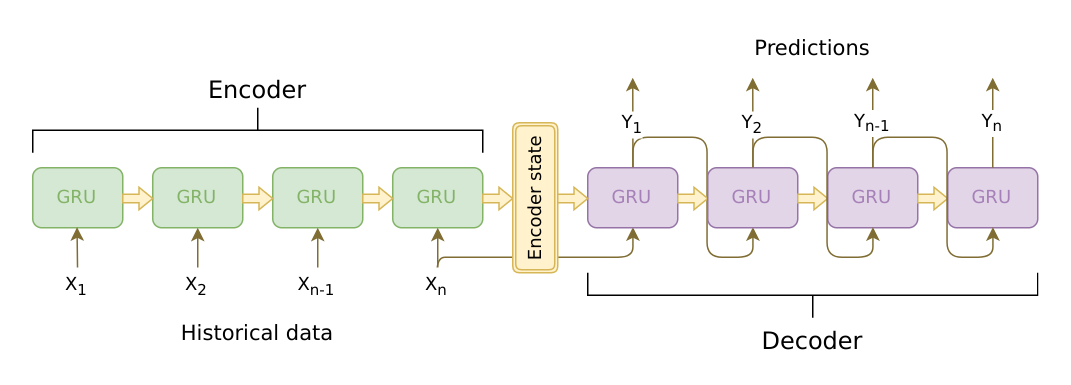
\includegraphics[width=\textwidth]{seq2seq}
	\caption*{Image source: \cite{seq2seq_eddy}}
\end{figure}
\end{itemize}

\section{Seq2seq with Attention}

\begin{itemize}
\item 
At each decoder step, it decides which source parts are more important

\item Concretely, at each $t,$:
	\begin{enumerate}[label=(\roman*)]
	\item
	Use previous token in RNN to update hidden state $h_t.$
	
	\item 
	Compute  $\score(h_t,s_k)$ between decoder hidden state $h_t$ and all encoder hidden states $s_1,\ldots,s_m;$
	
	\item 
	Compute attention weights: softmax attention scores;
	
	\item 
	Compute attention vector $a_t$: weighted sum of encoder states.
	
	\item 
	Use attention vector $a_t$ and hidden state $h_t$ in FNN to get output token.
	\end{enumerate}

\item Popular score functions:
	\begin{itemize}
	\item 
	Dot-product: $\score(h_t,s_k) = h_t^T s_k.$
	
	\item 
	Bilinear function: $\score(h_t,s_k) = h_t^T W s_k.$
	
	\item 
	Multi-layer perceptron: $\score(h_t,s_k) = v^T\tanh(W[h_t,s_k]).$
	\end{itemize}

\item Drawback: RNN is difficult to parallelize.

\begin{figure}[ht]
	\centering
	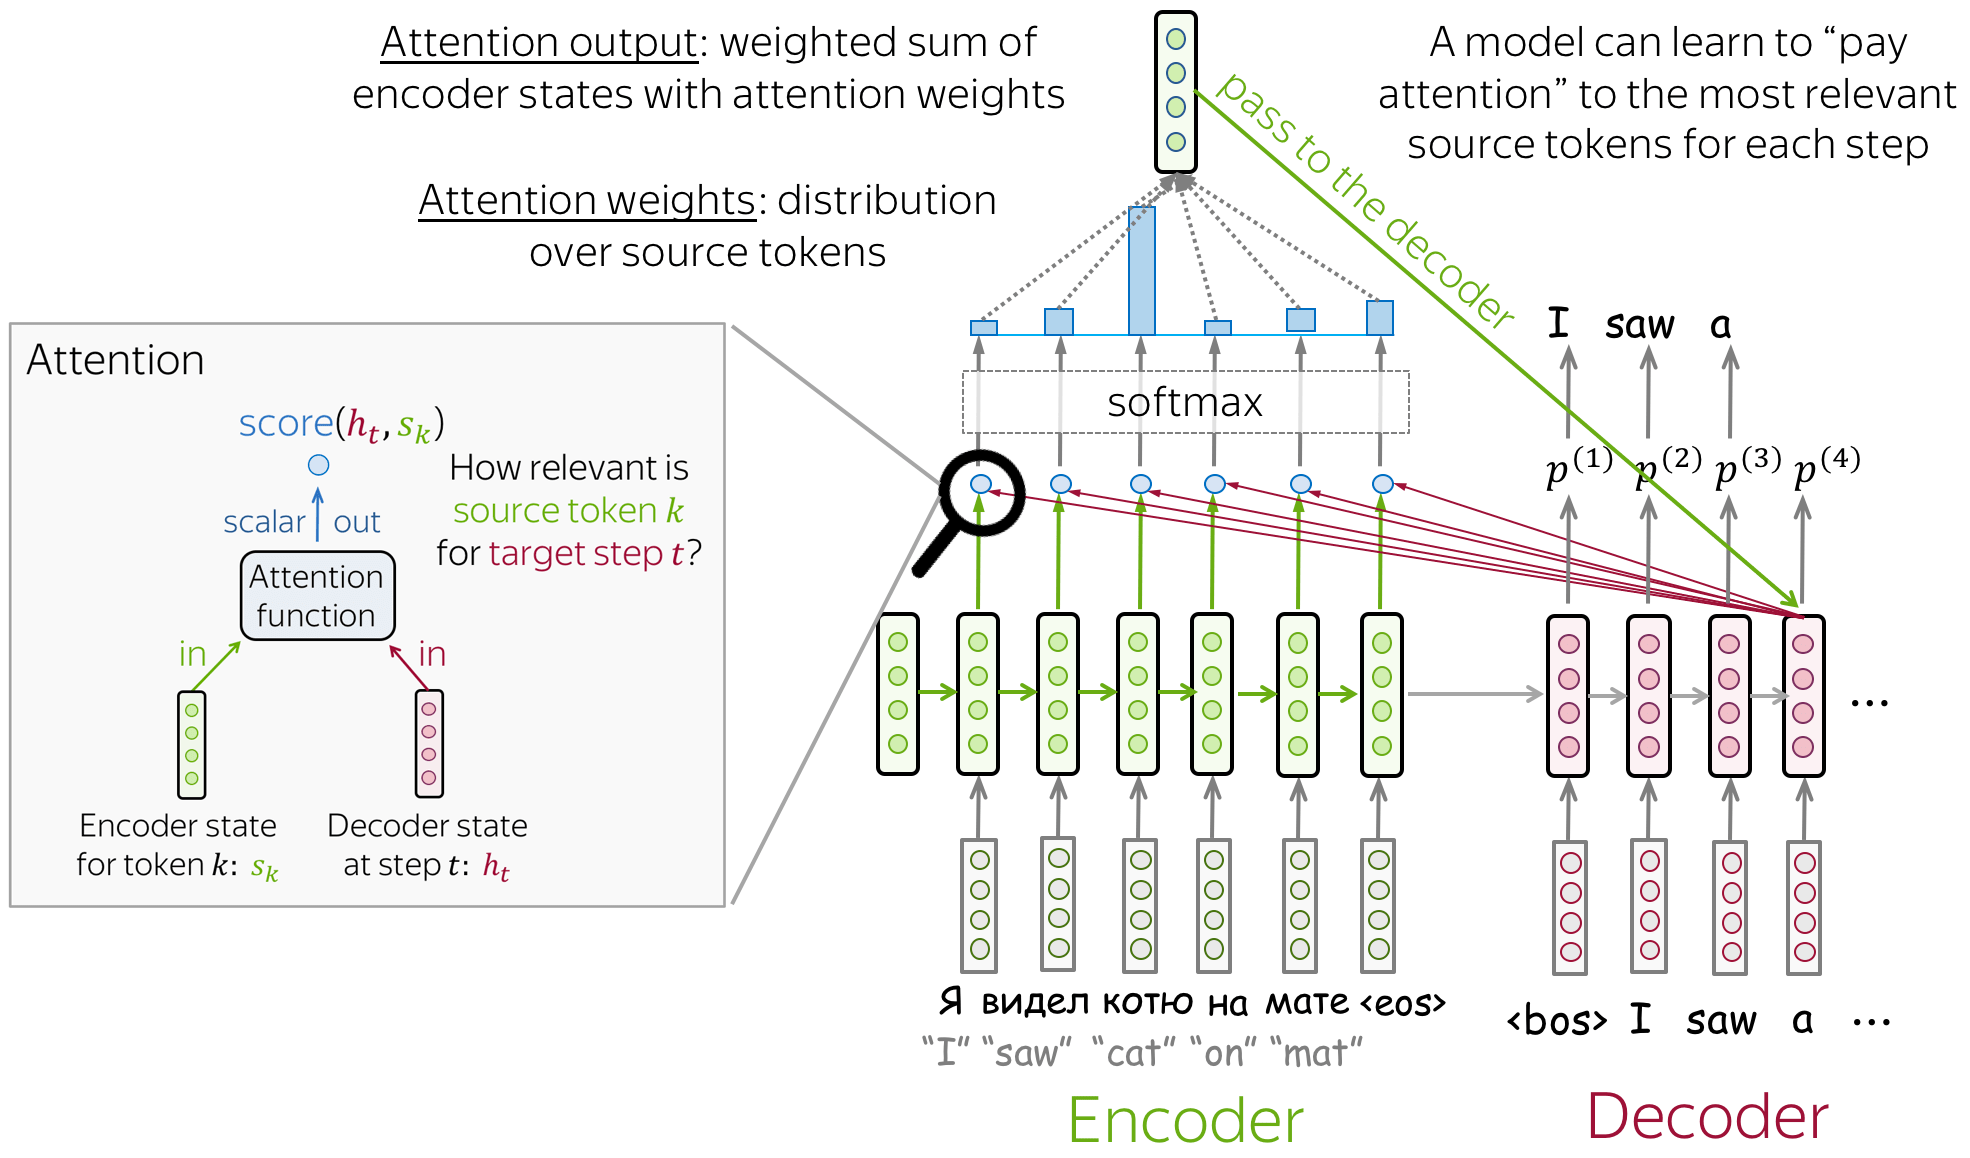
\includegraphics[width=\textwidth]{seq2seq_attention}
	\caption*{Image source: \cite{seq2seq_voita}}
\end{figure}
\end{itemize}

\section{Transformers}
\begin{itemize}
\item 
Encoding component is a stack (six in original paper) of encoders with same structure but different weights. Decoding component is a stack of decoders of the same number.

\item 
Encoders: Self-Attention \textrightarrow{} FNN
	\begin{itemize}
	\item 
	First encoder receives embedding of words.
	
	\item 
	Other encoders receive output of encoder directly below.
	\end{itemize}

\item 
Decoders: Self-Attention \textrightarrow{} Encoder-Decoder Attention \textrightarrow{} FNN
\end{itemize}

\subsection{Ingredients}
\subsubsection{Self-attention}
Process:
\begin{enumerate}
\item Create three vectors from each of the encoder’s input vectors: Query, Key, and Value vectors.

\item Note: in original paper, input vectors are in $\R^{512},$ and QKV vectors are in $\R^{64}.$

\item Self-attention score between $i$-th and $j$-th word is $q_i \cdot k_j$ for all $j.$

\item Divide scores by square root of dimension (8; this gives more stable gradients) and softmax.

\item Multiply each value vector $v_j$ by softmax scores.

\item Sum up the weighted value vectors. This is output of self-attention layer for $i$-th word.
\end{enumerate}
In matrix form, suppose our input is $X \in \R^{n \times d},$ where $n$ is the sequence length and $d$ is the embedding dimension. (So rows of $X$ are the inputs.) The QKV matrices are given by $W_Q, W_K, W_V \in \R^{d \times d_k}.$ Then the QKV vectors
\begin{align*}
    Q &= XW_Q \\
    K &= XW_K \\
    V &= XW_V
\end{align*}
are in $R^{n \times d_k}$
For each attention head, we have
\[ \att(Q,K,V) = \softmax\left(\frac{QK^T}{\sqrt{d_k}}\right) \times V \in \R^{n \times d_k}, \]
i.e., aggregate values weighted by attention.

\subsubsection{Multi-headed attention}
Do $h$ parallel attention heads, with different weight matrices for each head.
\[ \operatorname{MultiHead}(Q, K, V) = \operatorname{Concat}(\head_1, \ldots, \head_h) \times W_O, \]
where
\[ \head_i = \att(Q_i, K_i, V_i) \]
is output of each attention head and $W_O \in \R^{hd_k \times d}.$ Note that $\operatorname{MultiHead}(Q, K, V) \in \R^{n \times d}.$ 

\subsubsection{Positional encoding}
Transformers are permutation-invariant, so we add positional encoding to input embeddings.

\subsubsection{FNN}
Output of attention fed into FNN:
\[ \operatorname{FNN}(x) = \operatorname{ReLU}(xW_1 + b_1)W_2 + b_2. \]

\subsubsection{Residual connections \& layer normalization}
Each sub-layer (attention or feedforward) is followed by
\[ \layernorm(x + \operatorname{Sublayer}(x)). \]
Given $x \in \R^d,$ the layer norm is 
\[ \layernorm(x) = \frac{x - \mu}{\sqrt{\sigma^2 + \epsilon}} \cdot \gamma + \beta, \]
where
\begin{gather*}
    \mu = \frac{\sum x_i}{d} \text{ (mean over features)}\\
    \sigma^2 = \frac{\sum(x_i - \mu)^2}{d} \text{ (variance over features)}\\
    \gamma,\beta \text{: learned scaling and shifting parameters}\\
    \epsilon \text{: small constant to prevent division by zero}.
\end{gather*}

\subsection{Original Architecture}
Encoder Layer:
\begin{itemize}
    \item Input Embedding + Positional Encoding
    \item Multi-Head Self-Attention \textrightarrow{} Residual + Layer Norm
    \item Feed-Forward Network \textrightarrow{} Residual + Layer Norm
\end{itemize}
Decoder Layer:
\begin{itemize}
\item Masked Multi-Head Self-Attention (prevent peeking at future tokens)
\item Multi-Head Encoder-Decoder Attention \textrightarrow{} Residual + Layer Norm
\item Feed-Forward Network \textrightarrow{} Residual + Layer Norm
\end{itemize}

\subsection{Modern Architecture}
\begin{itemize}
    \item Input Embedding
    \item Layer Norm \textrightarrow{} Self-Attention \textrightarrow{} Residual
        \begin{itemize}
            \item Grouped-Query Attention
            \item Rotary Embeddings
        \end{itemize}
    \item Layer Norm \textrightarrow{} FNN \textrightarrow{} Residual
\end{itemize}

\subsubsection{Grouped-query attention}
\begin{itemize}
    \item Use same $W_K$ and $W_V$ across heads, and each head has its own $W_Q.$
    \item Better: divide heads into groups. Heads in the same group share $W_K$ and $W_V$
\end{itemize}

\subsubsection{Rotary positional embeddings}
\begin{itemize}
    \item Training done in batches, with fixed context size.
    \item Use padding for inputs smaller than context size.
    \item Instead, use separation token.
    \item Then rotary positional embeddings added to $Q$ and $K.$
\end{itemize}

\subsection{Other Techniques}
\subsubsection{Sparse attention}
Instead of global autoregressive self-attention, use local autoregressive self-attention in some layers.

\subsubsection{Mixture of experts (MOE)}
\begin{itemize}
    \item Instead of a single monolithic feedforward layer in the transformer block, use a set of expert networks, and route the input to only a few of them.
    \item A router (a smaller FNN) calculates which experts to turn on.
    \item Could do model merging by doing a weighted average of experts using weights from the router.
\end{itemize}

\end{document}